Nel paragrafo \ref{sec:chapter_tecnologie_abilitanti_webgl} è stato mostrato come nel browser venga utilizzato WebGL per usufruire dell’accelerazione grafica per il rendering 3D. 
Dal momento che, come per OpenGL, anche WebGL permette di interfacciarsi con le primitive solamente a basso livello, è necessario uno strumento che permetta di semplificare l’esperienza d’uso che altrimenti sarebbe fin troppo complessa, e Three.js è la soluzione a questo problema. Nonostante questa libreria contribuisca sensibilmente alla fruibilità di scene su browser, permangono tuttavia del problemi da risolvere: la scena deve avere una resa fotorealistica, e la fruizione della scena deve poter scalare su piattaforme multiple.
Per fruire di una scena, avendo anche la possibilità di navigarla, è necessario effettuare il rendering in real-time; questo vuol dire che ad ogni ciclo di rendering tutte le informazioni sulla scena devono essere ricalcolate.
Utilizzare Three.js per rendere una scena fotorealistica è una pressochè impossibile, perchè nonostante fornisca tutti gli strumenti per aumentare l’impatto grafico di una scena, sarebbe computazionalmente oneroso utilizzarli in un contesto real-time.
Nel capitolo \ref{cha:chapter_stato_arte} è stato mostrato come uno degli elementi principali per migliorare la resa visiva di una scena sia l’illuminazione indiretta, e come gli algoritmi di illuminazione indiretta siano onerosi da calcolare. 
Un supporto per il calcolo real-time dell’illuminazione indiretta sul renderer di three.js sarebbe quindi inutilizzabile sulla stragrande maggioranza delle piattaforme. Generalmente le prestazioni di un rendering real-time risentono del numero di luci in una scena; questo perchè con l’aumentare delle luci, aumenta la quantità di informazioni di luci e ombre che la fase di vertex shading deve computare ad ogni ciclo. 
Il fattore scalabilità è quindi fortemente influenzato dal numero di luci in una scena, specialmente in contesti come quello affrontato nel presente elaborato di tesi, dove si vogliono realizzare ambienti di dimensioni anche notevoli, come un’intera abitazione, e navigarli in prima persona. 

Per rendere scalabile il servizio di fruibilità della scena bisogna quindi ridurre il carico computazionale sulla pipeline di rendering, rendendola appunto “lightweight”, pur mantenendo la resa grafica fotorealistica.
\\
A fronte di tale necessità verranno descritti gli accorgimenti adottati per velocizzare il ciclo di render.
Il primo accorgimento è quello di liberare la pipeline di rendering dal calcolo delle informazioni luminose, le quali verranno preprocessate offline una sola volta, e memorizzate all’interno di strutture dati chiamate \textbf{lightmapped texture} mediante il processo di baking; nel capitolo \ref{sec:chapter_lrl_li_te_ba} verrà spiegato cosa sono le lightmapped texture e quali caratteristiche la differenziano da una normale lightmap. 
\\
Siccome il calcolo dell’illuminazione non dipende più dal renderer di ThreeJS, può essere affidato ad uno strumento esterno, come un’applicazione desktop in grado di processare algoritmi di illuminazione complessi; ovviamente dovrà anche essere in grado di memorizzare i risultati ottenuti, processo di baking delle lightmap.
\\
Un’altro dettaglio che incide profondamente sulle performance di un rendering è la presenza di effetti rifrangenti o riflettenti all’interno della scena. Ad esempio Three.js permette di creare degli specchi che riflettono l’ambiente circostante renderizzandolo in tempo reale.
Se all’interno della scena ci fossero degli oggetti in movimento, questi apparirebbero riflessi nella posizione in cui effettivamento si trovano.
\\
\begin{figure}[htb]
 \centering
 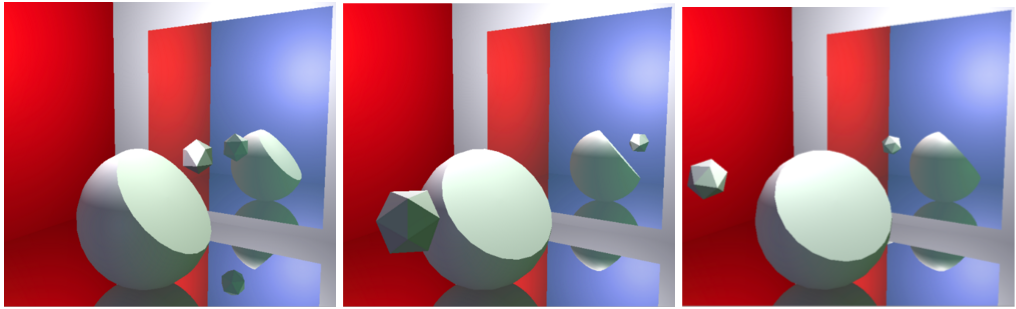
\includegraphics[width=0.8\linewidth]{images/chapter_lrl/lrl_specchio.png}\hfill
 \caption[ThreeJS Mirror]{In foto è possibile notare come lo specchio realizzato in ThreeJS rifletta in ogni istante di tempo gli oggetti della scena nelle posizioni in cui effettivamente si trovano.}
 \label{fig:lrl_specchio}
\end{figure}
Nonostante il comportamento assolutamente realistico gli specchi risultano inutilizzabili se si vuole  alleggerire il carico di lavoro del renderer. Questo perchè per ogni specchio aggiunto una nuova pipeline di rendering dovrà essere eseguita, aumentando drasticamente la mole di lavoro da svolgere. Questa è sicuramente la soluzione meno scalabile perchè all’aumentare del numero degli specchi ci sarà bisogno di un hardware sempre più potente per mantenere fluida l’esperienza visiva. Se il contesto di utilizzo prevede scene prevalentemente statiche, è possibile  mantenere un’unica pipeline di rendering pur avendo effetti riflettenti o rifrangenti, utilizzando delle env-map. 
\\
Nel paragrafo \ref{sec:chapter_lrl_cond_app} verrano mostrate le condizioni che una scena deve soddisfare affichè il suo render possa essere reso leggero dalle soluzioni sopra mostrate.
